\documentclass[a4paper,12pt]{article}

\usepackage[french]{babel}
\usepackage[T1]{fontenc} 
\usepackage[latin1]{inputenc}
\usepackage{graphicx}
%\usepackage{amsmath}

\author{R�mi Synave, Stefka Gueorguieva, Pascal Desbarats}
\title{Manuel de la biblioth�que SUBDIVISION}
\date{}

\begin{document}
\maketitle

\section{Utilisation}
Dans cette biblioth�que est impl�ment�e la subdivision loop.\\

\section{Fonctions}


\textbullet void vf\_model\_loop(vf\_model *m, int nbiter)\\
Subdivision d'un \textit{vf\_model} avec la m�thode de Loop \cite{L1987}.\\
Algorithme :\\
1) Cr�ation d'une nouvelle liste de sommets et d'une nouvelle liste de faces.\\
2) Ajout d'un sommet au milieu de toutes les ar�tes (voir figure \ref{decouparete_vf_model_loop}) -> D�coupage des ar�tes en deux. L'index du sommet au milieu de l'arete est mis dans la variable \textit{midvertex} de la \textit{vf\_edge}.\\
\begin{figure}[htbp]
\centering
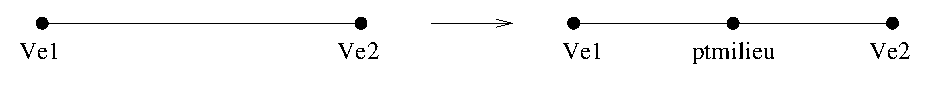
\includegraphics[width=10cm]{./images/decouparete_vf_model_loop.eps}
\caption{Ajout d'un sommet sur les aretes.}
\label{decouparete_vf_model_loop}
\end{figure}
3) D�coupage des faces (ve1,ve2,ve3) en quatre faces (voir figure \ref{decoupface_vf_model_loop}) :\\
\begin{itemize}
\item (ve1,ptmilieu1,ptmilieu2)
\item (ptmilieu1,ve2,ptmilieu3)
\item (ptmilieu2,ptmilie3,ve3)
\item (ptmilieu3,ptmilieu2,ptmilieu1)
\end{itemize}
\begin{figure}[htbp]
\centering
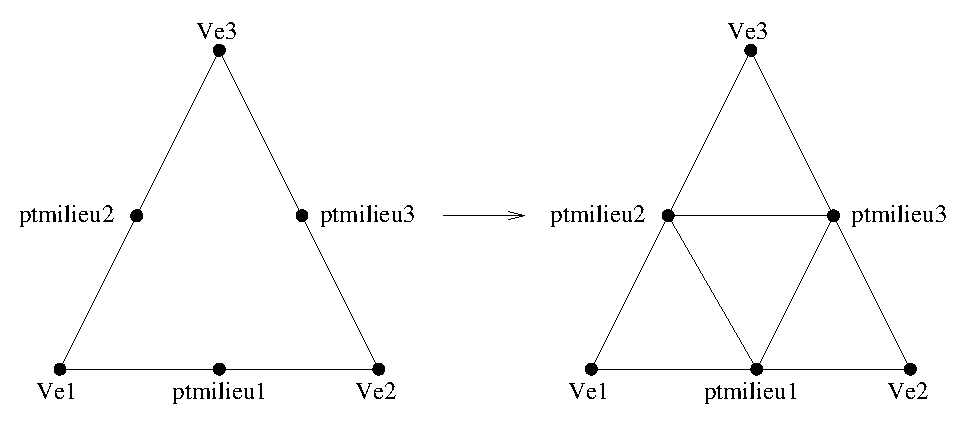
\includegraphics[width=10cm]{./images/decoupface_vf_model_loop.eps}
\caption{D�coupage des faces.}
\label{decoupface_vf_model_loop}
\end{figure}
4) Repositionnement des sommets existant avant le d�coupage des ar�tes puis des nouveaux sommets. (voir figure \ref{repositionnement_vf_model_loop})\\
\begin{figure}[htbp]
\centering
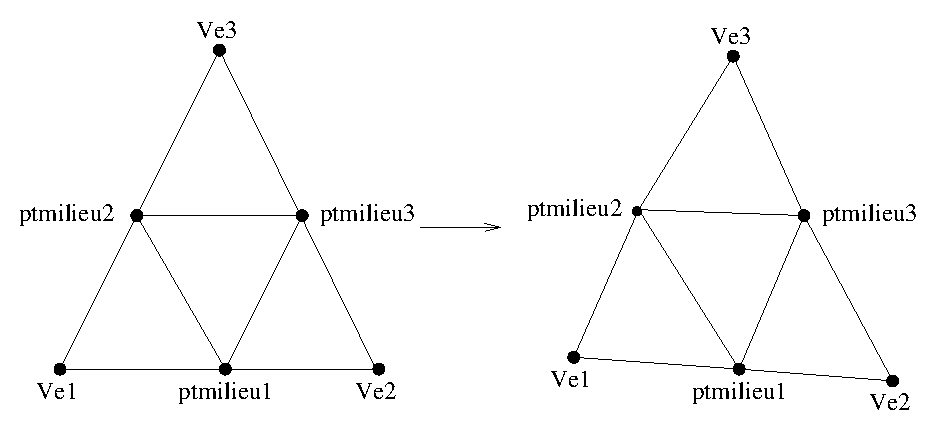
\includegraphics[width=10cm]{./images/repositionnement_vf_model_loop.eps}
\caption{Repositionnement des sommets.}
\label{repositionnement_vf_model_loop}
\end{figure}



\textbullet void vef\_model\_loop(vef\_model *m, int nbiter)\\
Subdivision d'un \textit{vef\_model} avec la m�thode de Loop \cite{L1987}.\\
Algorithme :\\
1) Cr�ation d'une nouvelle liste de sommets, d'un nouvelle liste d'aretes et d'une nouvelle liste de faces.\\
2) Ajout d'un sommet au milieu de toutes les ar�tes (voir figure \ref{decouparete_vef_model_loop}) -> D�coupage des ar�tes en deux. Les sommets cr��s ont comme index \textit{nombre\_de\_sommets\_du\_mod�le+index\_de\_l\_arete}.\\
\begin{figure}[htbp]
\centering
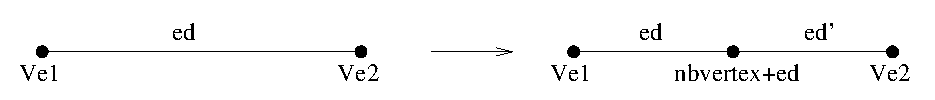
\includegraphics[width=10cm]{./images/decouparete_vef_model_loop.eps}
\caption{Ajout d'un sommet sur les aretes.}
\label{decouparete_vef_model_loop}
\end{figure}
3) D�coupage des faces en quatre faces (voir figure \ref{decoupface_vef_model_loop}).\\
\begin{figure}[htbp]
\centering
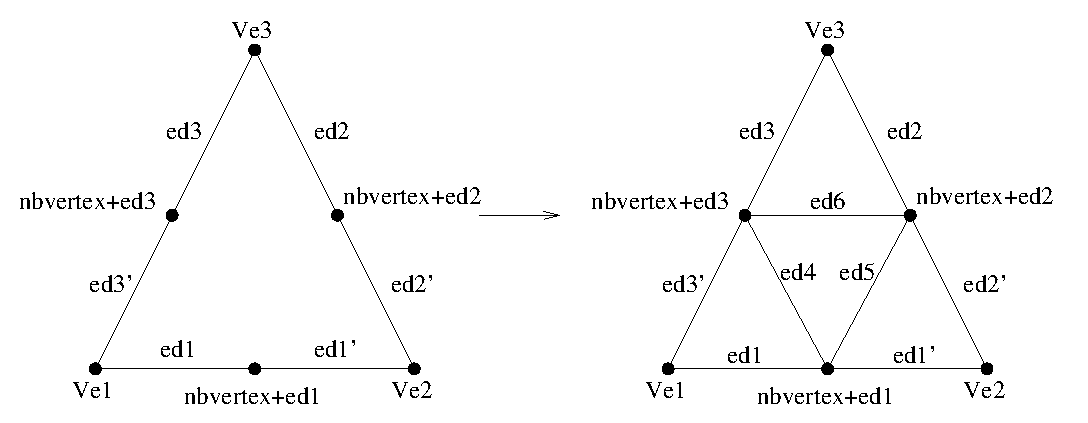
\includegraphics[width=10cm]{./images/decoupface_vef_model_loop.eps}
\caption{D�coupage des faces.}
\label{decoupface_vef_model_loop}
\end{figure}
4) Repositionnement des sommets existant avant le d�coupage des ar�tes puis des nouveaux sommets. (voir figure \ref{repositionnement_vef_model_loop})\\
\begin{figure}[htbp]
\centering
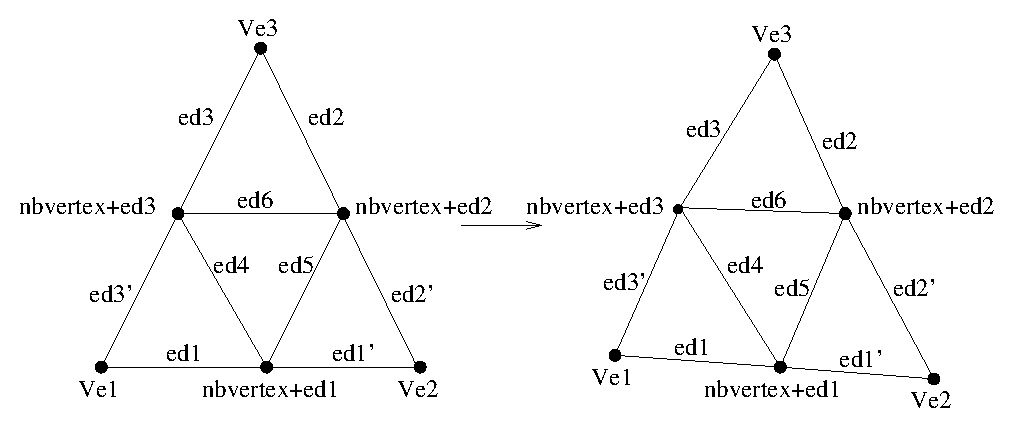
\includegraphics[width=10cm]{./images/repositionnement_vef_model_loop.eps}
\caption{Repositionnement des sommets.}
\label{repositionnement_vef_model_loop}
\end{figure}

\bibliographystyle{unsrt}
\bibliography{manuel}

\end{document}
